
%*----------- SLIDE -------------------------------------------------------------
\begin{frame}[t]{A abordagem}
  \transboxout[duration=0.5]
  \framesubtitle{Diagrama}

  % Define block styles
  \tikzstyle{decision} = [diamond, draw, fill=blue!20,
  text width=4.5em, text badly centered, node distance=3cm, inner sep=0pt]
  \tikzstyle{block} = [rectangle, draw, fill=blue!20,
  text width=5em, text centered, rounded corners, minimum height=4em, node distance=3cm]
  \tikzstyle{line} = [draw, -latex']
  \tikzstyle{cloud} = [draw, ellipse,fill=red!20, node distance=3cm,
  minimum height=2em]

  \begin{center}
    \begin{tikzpicture}[node distance = 2cm, auto]
      % Place nodes
      \node [block] (mec) {Estrutura Mecânica};
      \node [block, right of=mec] (kinematic) {Modelo Cinemático};
      \node [block, right of=kinematic] (dynamic) {Modelo Dinâmico};
      \node [block, right of=dynamic] (motors) {Modelo dos Motores};
      \node [block, right of=motors] (param) {Estimativa dos Parâmetros};
  
      % \node [cloud, left of=mec] (init) {init};
      % \node [block, below of=init] (identify) {identify candidate models};
      % \node [block, below of=identify] (evaluate) {evaluate candidate models};
      % \node [block, left of=evaluate, node distance=3cm] (update) {update model};
      % \node [decision, below of=evaluate] (decide) {is best candidate better?};
      % \node [block, below of=decide, node distance=3cm] (stop) {stop};
  
      % Draw edges
      \path [line] (mec) -- (kinematic);
      \path [line] (kinematic) -- (dynamic);
      \path [line] (dynamic) -- (motors);
      \path [line] (motors) -- (param);
      % \path [line] (evaluate) -- (decide);
      % \path [line] (decide) -| node [near start] {yes} (update);
      % \path [line] (update) |- (identify);
      % \path [line] (decide) -- node {no}(stop);
      % \path [line] (system) -- (init);
      % \path [line,dashed] (system) |- (evaluate);
    \end{tikzpicture}
  \end{center}

  %*----------- notes
  \note[item]{Notes can help you to remember important information. Turn on the notes option.}
\end{frame}

%*----------- SLIDE -------------------------------------------------------------
\begin{frame}[c]{A abordagem}
  \framesubtitle{Estrutura Mecânica}
  \transdissolve[duration=0.5]

  \begin{figure}[ht!]
    \centering
    \begin{subfigure}[b]{0.38\textwidth}
      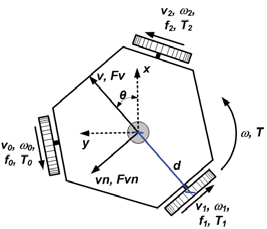
\includegraphics[width=\textwidth]{three_wheeled_robot_geometry.png}
      \caption{Três rodas.}
      \label{fig:3_wheels_robot_geometry}
    \end{subfigure}
    ~
    \begin{subfigure}[b]{0.38\textwidth}
      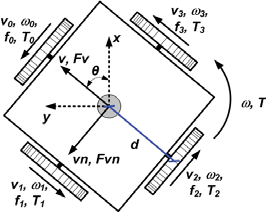
\includegraphics[width=\textwidth]{four_wheeled_robot_geometry.png}
      \caption{Quatro rodas.}
      \label{fig:4_wheels_robot_geometry}
    \end{subfigure}
    
    \caption{Estrutura geométrica de ambas as configurações do robô. \cite{Oliveira2008}}
  \end{figure}


  %*----------- notes
  \note[item]{Notes can help you to remember important information. Turn on the notes option.}
\end{frame}

%*----------- SLIDE -------------------------------------------------------------
\begin{frame}[c]{A abordagem}
  \framesubtitle{Modelo Cinemático}
  \transdissolve[duration=0.5]

  \begin{figure}[ht!]
    \centering

    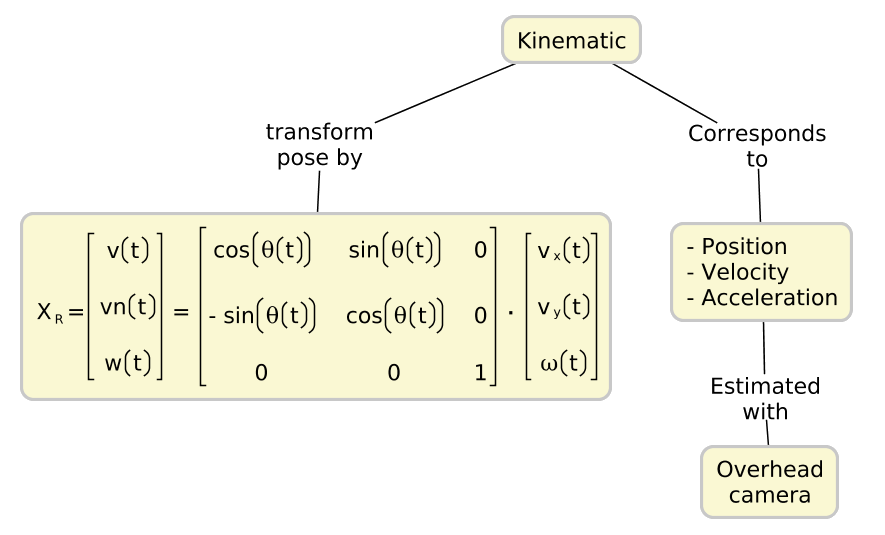
\includegraphics[width=0.75\textwidth]{kinematic_cmap.png}
    \label{fig:kinematic_cmap}

  \end{figure}


  %*----------- notes
  \note[item]{Notes can help you to remember important information. Turn on the notes option.}
\end{frame}

%*----------- SLIDE -------------------------------------------------------------
\begin{frame}[t]{A abordagem}
  \transboxout[duration=0.5]
  \framesubtitle{Modelo Cinemático: 3 rodas}
  \begin{columns}
    \column{.4\textwidth}
    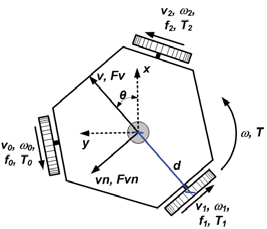
\includegraphics[width=\textwidth]{three_wheeled_robot_geometry.png}
    \column{.4\textwidth}
      \begin{equation*}
        v(t) = 
        \frac{\sqrt{3}}{3} \cdot
        \left(
          {\color[rgb]{1,0,0} v_2(t)} - 
          {\color[rgb]{0,0.5,0.5} v_0(t)}
        \right)
      \end{equation*}

      \begin{equation*}
        vn(t) =
        \frac{1}{3} \cdot
        \left(
          {\color[rgb]{1,0,0} v_2(t)} -
          {\color[rgb]{0,0.5,0.5} v_0(t)}\right) - 
          \frac{2}{3} \cdot
          {\color[rgb]{0,0,1} v_1(t)}
      \end{equation*}

      \begin{equation*}
        \omega(t) =
        \frac{1}{3d}\cdot
        \left(
          {\color[rgb]{0,0.5,0.5} v_0(t)} +
          {\color[rgb]{0,0,1} v_1(t)} +
          {\color[rgb]{1,0,0} v_2(t)}
        \right)
      \end{equation*}
  \end{columns}
  %*----------- notes
  \note[item]{Notes can help you to remember important information. Turn on the notes option.}
\end{frame}


%*----------- SLIDE -------------------------------------------------------------
\begin{frame}[t]{A abordagem}
  \transboxout[duration=0.5]
  \framesubtitle{Modelo Cinemático: 4 rodas}
  \begin{columns}
    \column{.4\textwidth}
    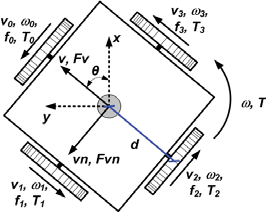
\includegraphics[width=\textwidth]{four_wheeled_robot_geometry.png}
    \column{.5\textwidth}
      \begin{equation*}
        v(t) = 
        \frac{1}{2} \cdot
        \left(
          {\color[rgb]{1,0,0} v_3(t)} - 
          {\color[rgb]{0,0.5,0.5} v_1(t)}
        \right)
      \end{equation*}

      \begin{equation*}
        vn(t) = 
        \frac{1}{2} \cdot
        \left(
          {\color[rgb]{1,0,1} v_0(t)} - 
          {\color[rgb]{0,0,1} v_2(t)}
        \right)
      \end{equation*}

      \begin{equation*}
        \omega(t) =
        \frac{1}{4d}\cdot
        \left(
          {\color[rgb]{1,0,1} v_0(t)} + 
          {\color[rgb]{0,0.5,0.5} v_1(t)} +
          {\color[rgb]{0,0,1} v_2(t)} +
          {\color[rgb]{1,0,0} v_3(t)} 
        \right)
      \end{equation*}
  \end{columns}
  %*----------- notes
  \note[item]{Notes can help you to remember important information. Turn on the notes option.}
\end{frame}


%*----------- SLIDE -------------------------------------------------------------
\begin{frame}[c]{A abordagem}
  \framesubtitle{Modelo Dinâmico}
  \transdissolve[duration=0.5]

  \begin{figure}[ht!]
    \centering

    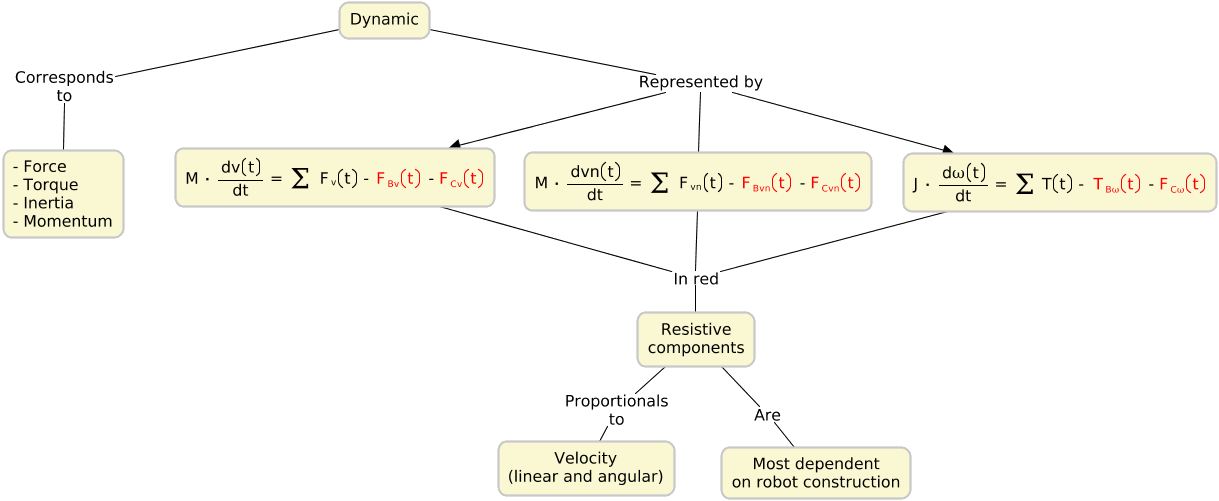
\includegraphics[width=\textwidth]{dynamic_cmap.png}
    \label{fig:dynamic_map}

  \end{figure}


  %*----------- notes
  \note[item]{Notes can help you to remember important information. Turn on the notes option.}
\end{frame}

%*----------- SLIDE -------------------------------------------------------------
\begin{frame}[t]{A abordagem}
  \transboxout[duration=0.5]
  \framesubtitle{Modelo Dinâmico: 3 rodas}
  \begin{columns}
    \column{.4\textwidth}
    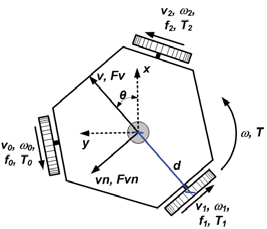
\includegraphics[width=\textwidth]{three_wheeled_robot_geometry.png}
    \column{.6\textwidth}
      \begin{equation*}
        \sum F_v(t) = 
        \sin \left( \frac{\pi}{3} \right) \cdot
        \left(
          {\color[rgb]{1,0,0} F_2(t)} - 
          {\color[rgb]{0,0.5,0.5} F_0(t)}
        \right)
      \end{equation*}

      \begin{equation*}
        \sum F_{vn}(t) =
        \cos \left( \frac{\pi}{3} \right) \cdot
        \left(
          {\color[rgb]{1,0,0} F_2(t)} +
          {\color[rgb]{0,0.5,0.5} F_0(t)}
        \right) - 
        {\color[rgb]{0,0,1} F_1(t)}
      \end{equation*}

      \begin{equation*}
        \sum T(t) =
        d \cdot
        \left(
          {\color[rgb]{0,0.5,0.5} F_0(t)} +
          {\color[rgb]{0,0,1} F_1(t)} +
          {\color[rgb]{1,0,0} F_2(t)}
        \right)
      \end{equation*}
  \end{columns}
  %*----------- notes
  \note[item]{Notes can help you to remember important information. Turn on the notes option.}
\end{frame}

\begin{frame}[t]{A abordagem}
  \transboxout[duration=0.5]
  \framesubtitle{Modelo Dinâmico: 4 rodas}
  \begin{columns}
    \column{.4\textwidth}
    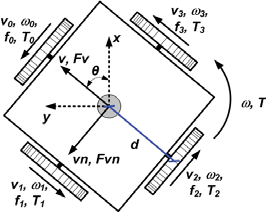
\includegraphics[width=\textwidth]{four_wheeled_robot_geometry.png}
    \column{.5\textwidth}
      \begin{equation*}
        \sum F_v(t) = 
        \left(
          {\color[rgb]{1,0,0} F_3(t)} - 
          {\color[rgb]{0,0.5,0.5} F_1(t)}
        \right)
      \end{equation*}

      \begin{equation*}
        \sum F_{vn}(t) = 
        \left(
          {\color[rgb]{1,0,1} F_0(t)} - 
          {\color[rgb]{0,0,1} F_2(t)}
        \right)
      \end{equation*}

      \begin{equation*}
        \sum T(t) = 
        d\cdot
        \left(
          {\color[rgb]{1,0,1} F_0(t)} + 
          {\color[rgb]{0,0.5,0.5} F_1(t)} +
          {\color[rgb]{0,0,1} F_2(t)} +
          {\color[rgb]{1,0,0} F_3(t)} 
        \right)
      \end{equation*}
  \end{columns}
  %*----------- notes
  \note[item]{Notes can help you to remember important information. Turn on the notes option.}
\end{frame}

%*----------- SLIDE -------------------------------------------------------------
\begin{frame}[c]{A abordagem}
  \framesubtitle{Modelo dos Motores}
  \transdissolve[duration=0.5]

  \begin{figure}[ht!]
    \centering

    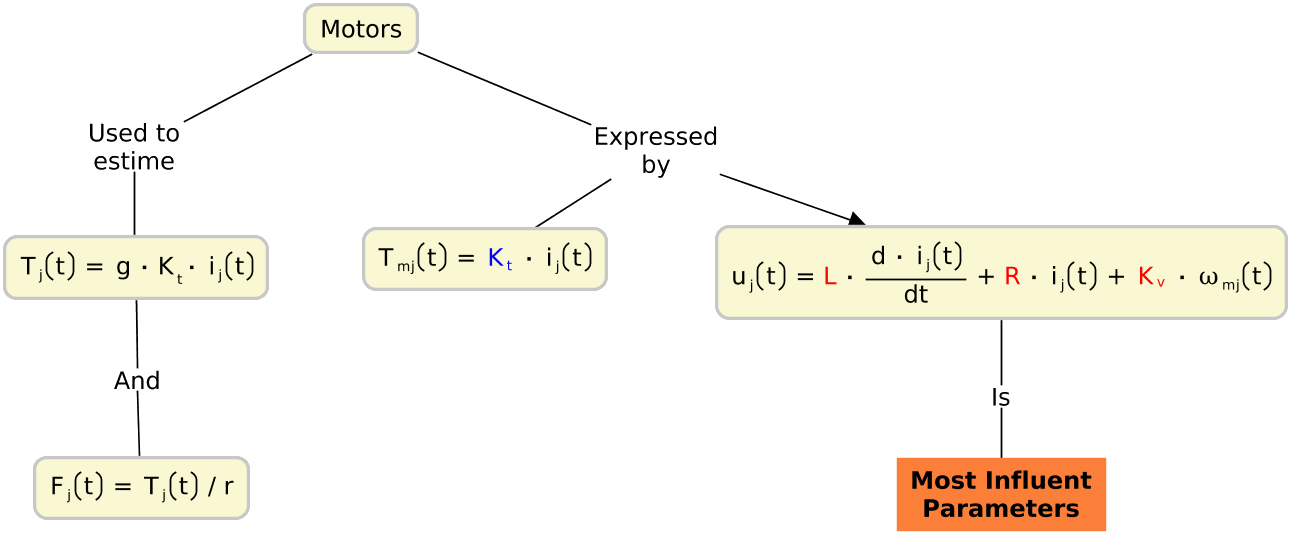
\includegraphics[width=\textwidth]{motor_cmap.png}
    \label{fig:motor_cmap}

  \end{figure}


  %*----------- notes
  \note[item]{Notes can help you to remember important information. Turn on the notes option.}
\end{frame}

%*----------- SLIDE -------------------------------------------------------------
\begin{frame}[c]{A abordagem}
  \framesubtitle{Estimativa dos Parâmetros}
  \transdissolve[duration=0.5]

  \begin{figure}[ht!]
    \centering

    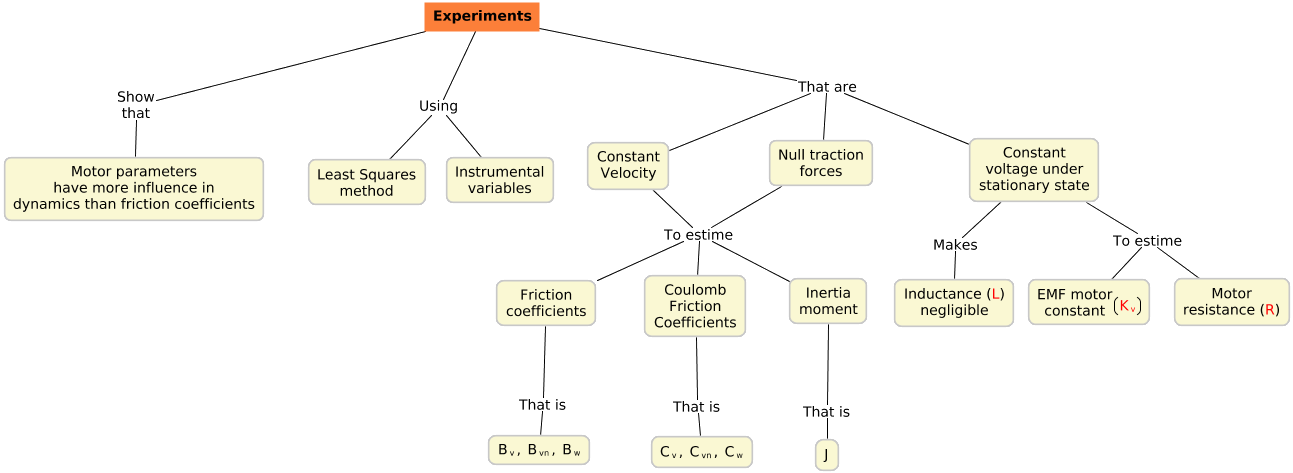
\includegraphics[width=1.05\textwidth]{experiments_cmap.png}
    \label{fig:experiments}

  \end{figure}


  %*----------- notes
  \note[item]{Notes can help you to remember important information. Turn on the notes option.}
\end{frame}